\section{Ergebnisse}
\label{sec:ergebnisse}
In diesem Abschnitt werden die Ergebnisse der Datenauswertung wiedergegeben und interpretiert.
Die Auswertungen der verschiedenen Studien haben gezeigt, dass Code-Metriken mit Sicherheitslücken auf statistisch signifikanten Niveau\cite{chowdhury_zulkernine_2010,chowdhury_zulkernine_2009,alves_et_al}.

Chowdhury und Zulkernine \cite{chowdhury_zulkernine_2010} zeigen, dass die CCC-Metriken im Durchschnitt eine Korrelation von 0.5 aufweisen mit einem p-Wert < 0.05.
Dies bestätigt die erste Hypothese auf Abschnitt \ref{sec:hypothesen}.
\begin{figure}
	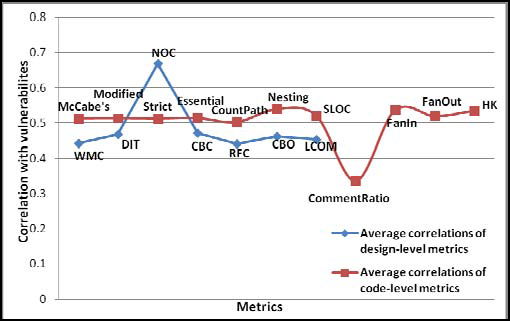
\includegraphics[width=\textwidth]{img/code_vs_design.png}
	\label{fig:code_vs_design}
	\caption{Durchschnittliche Korrelation mit Sicherheitslücken für gegebene Metriken; Einteilung nach Code-Level und Design-Level}
\end{figure}
Abbildung \ref{fig:code_vs_design} zeigt, inwieweit die einzelnen Metriken von der durchschnittlichen Korrelation der jeweiligen Gruppe (Code-Level bzw. Design-Level) abweichen.
Es konnte festgestellt werden, dass die Anzahl der Unterklassen ("`Number of Children"') die höchste Korrelation mit Sicherheitslücken aufweist, während das Verhältnis von Quellcode zu Kommentaren nur schwach korreliert.
Zusätzlich konnte festgestellt werden, dass die Verteilung der Korrelationen über mehrere Versionen von Mozilla Firefox hinweg konsistent ist.
